\documentclass[11pt]{beamer}
\usetheme{Boadilla}
\usepackage[utf8]{inputenc}
\usepackage{amsmath}
\usepackage{amsfonts}
\usepackage{amssymb}
\usepackage{graphicx}
\usepackage{tabularx}
\usepackage{tikz}
\usetikzlibrary{arrows,shapes.geometric,positioning}
\usepackage{pifont}% http://ctan.org/pkg/pifont
\newcommand{\xmark}{\ding{55}}%
% Define block styles
\tikzstyle{block} = [rectangle, draw, fill=blue!20, 
    text width=9.5em, text centered, rounded corners, minimum height=4em]
\tikzstyle{line} = [draw, -latex]

\graphicspath{{fig/}}

\author[Weiyao Ke]{Weiyao Ke, J Scott Moreland, Jonah E Bernhard, and Steffen A Bass}
\title[3D Initial Condition]{Constrain Initial 3D Entropy Production in Relativistic heavy-ion collisions from $p$-Pb and Pb-Pb Collisions. \\
\vspace*{0.1cm}
\small PRC 96, 044912 (2017) }

%\setbeamercovered{transparent}
%\setbeamertemplate{navigation symbols}{}
\usepackage{pgf}
\logo{\pgfputat{\pgfxy(0,7.7)}{\pgfbox[right,base]{
\includegraphics[height=1cm]{qcdlogo.pdf}}}}
%\newcommand{\nologo}{\setbeamertemplate{logo}{}}

\institute{Duke University}
\date{\today}
\newcommand{\TRENTo}{T\raisebox{-0.2em}{R}ENTo~}
\begin{document}

\begin{frame}
\titlepage
\end{frame}

\section{Initial condition of heavy-ion collisions}
\begin{frame}{Initial condition of heavy ion collision}
\begin{itemize}
\item Dynamical models of heavy-ion collision (hydrodynamics and other dynamical models), require an initial condition to start.\\
\begin{center}
Hydro: energy/entropy density, fluid velocity, ...
\end{center}
\item Their uncertainties propagate to the extraction of QGP properties.
\vspace*{0.3cm}
\item There are continuous progresses in first principal calculation of 2D (beam direction invariant) and 3D initial condition, but very hard.
\vspace*{0.3cm}
\item Just look at entropy density. How / what can we learn from data about 3D entropy production?
\begin{center}
\colorbox{orange!40}{Systemically comparing a parametric model to data.}
\end{center}
\end{itemize}
\end{frame}

\begin{frame}{When beam direction evolution becomes important.}
\begin{itemize}
\item Looking at midrapidity in A-A, usually assume invariance in beam direction ($\eta$).
\item Rapidity dependent observables necessitate a 3D initial condition.
\item In small system ($p$-A): strong asymmetry in beam direction.
\end{itemize}

\begin{overprint}
\onslide<1>
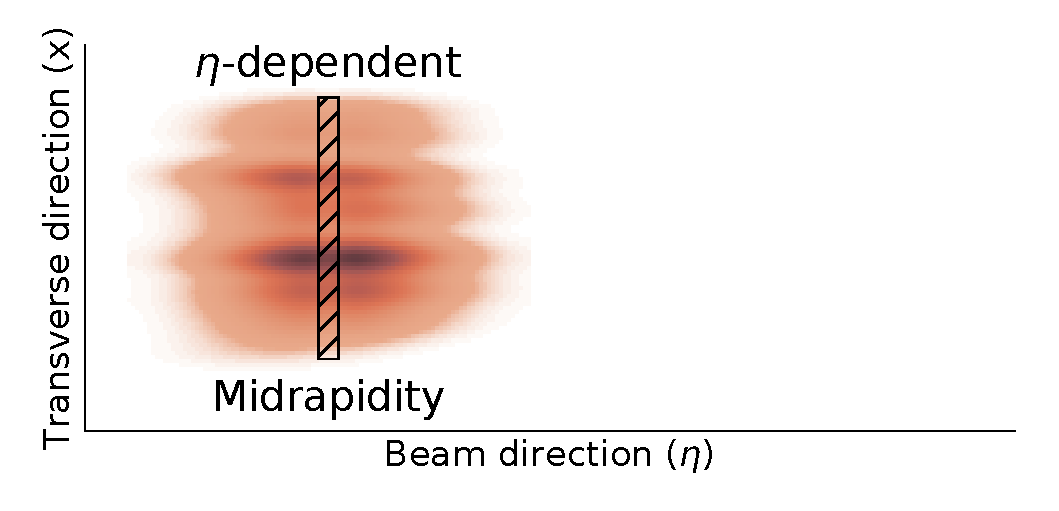
\includegraphics[width=0.67\textwidth]{nuclei_demo_a.pdf}
\onslide<2>
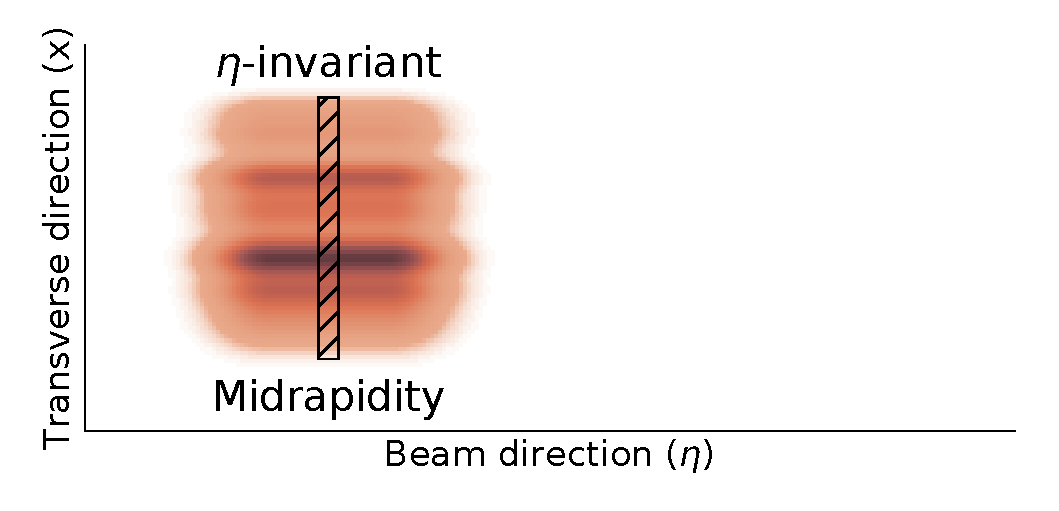
\includegraphics[width=0.67\textwidth]{nuclei_demo_b.pdf}
\onslide<3>
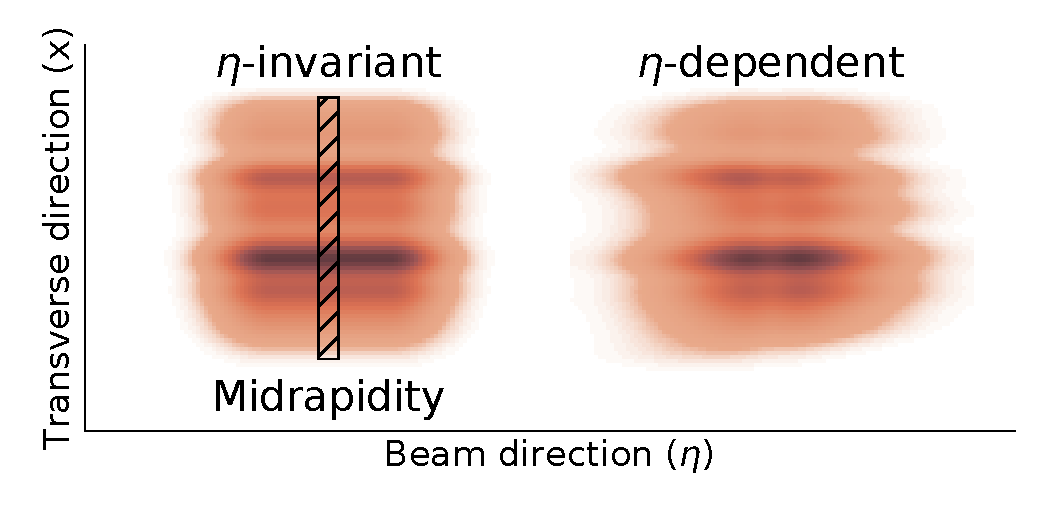
\includegraphics[width=0.67\textwidth]{nuclei_demo_01.pdf}
\onslide<4>
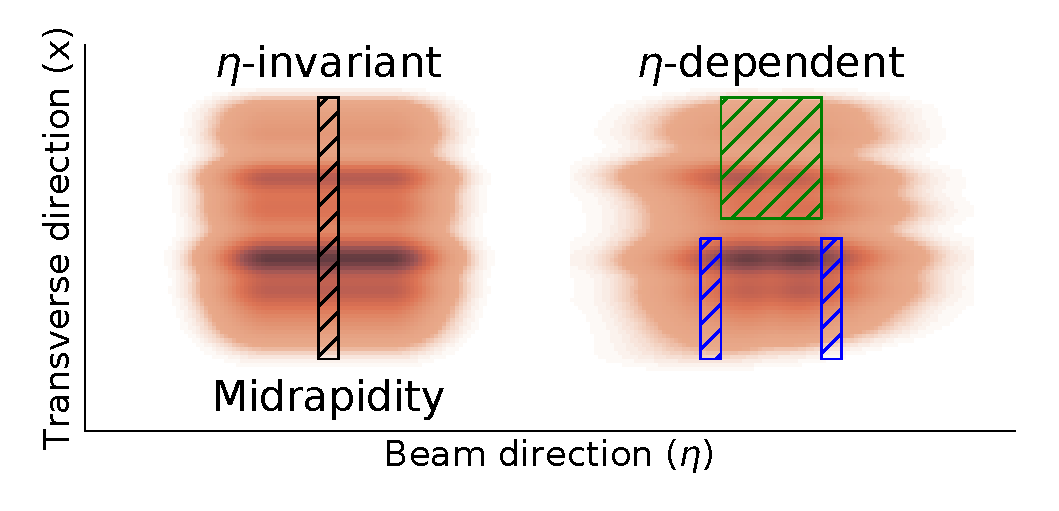
\includegraphics[width=0.67\textwidth]{nuclei_demo_02.pdf}
\onslide<5->
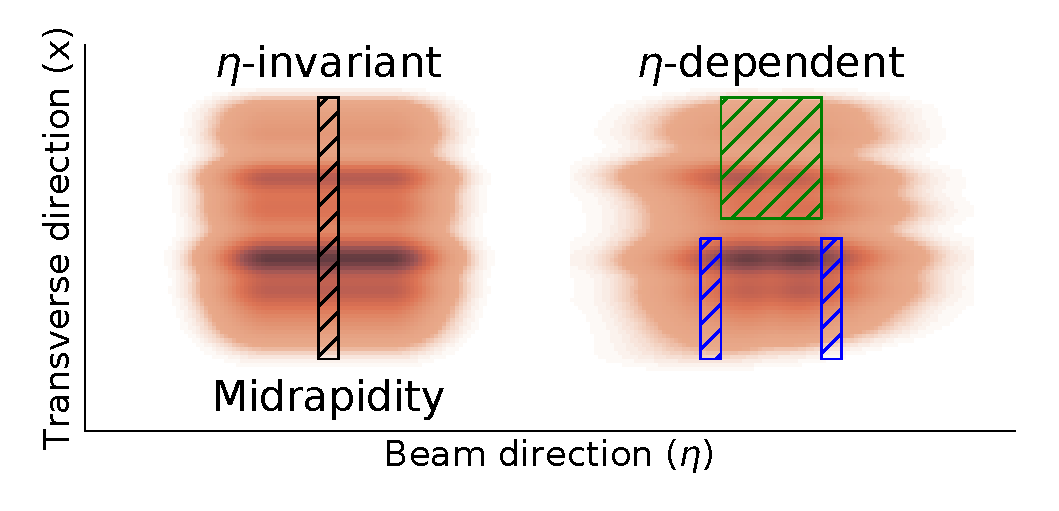
\includegraphics[width=0.67\textwidth]{nuclei_demo_02.pdf}
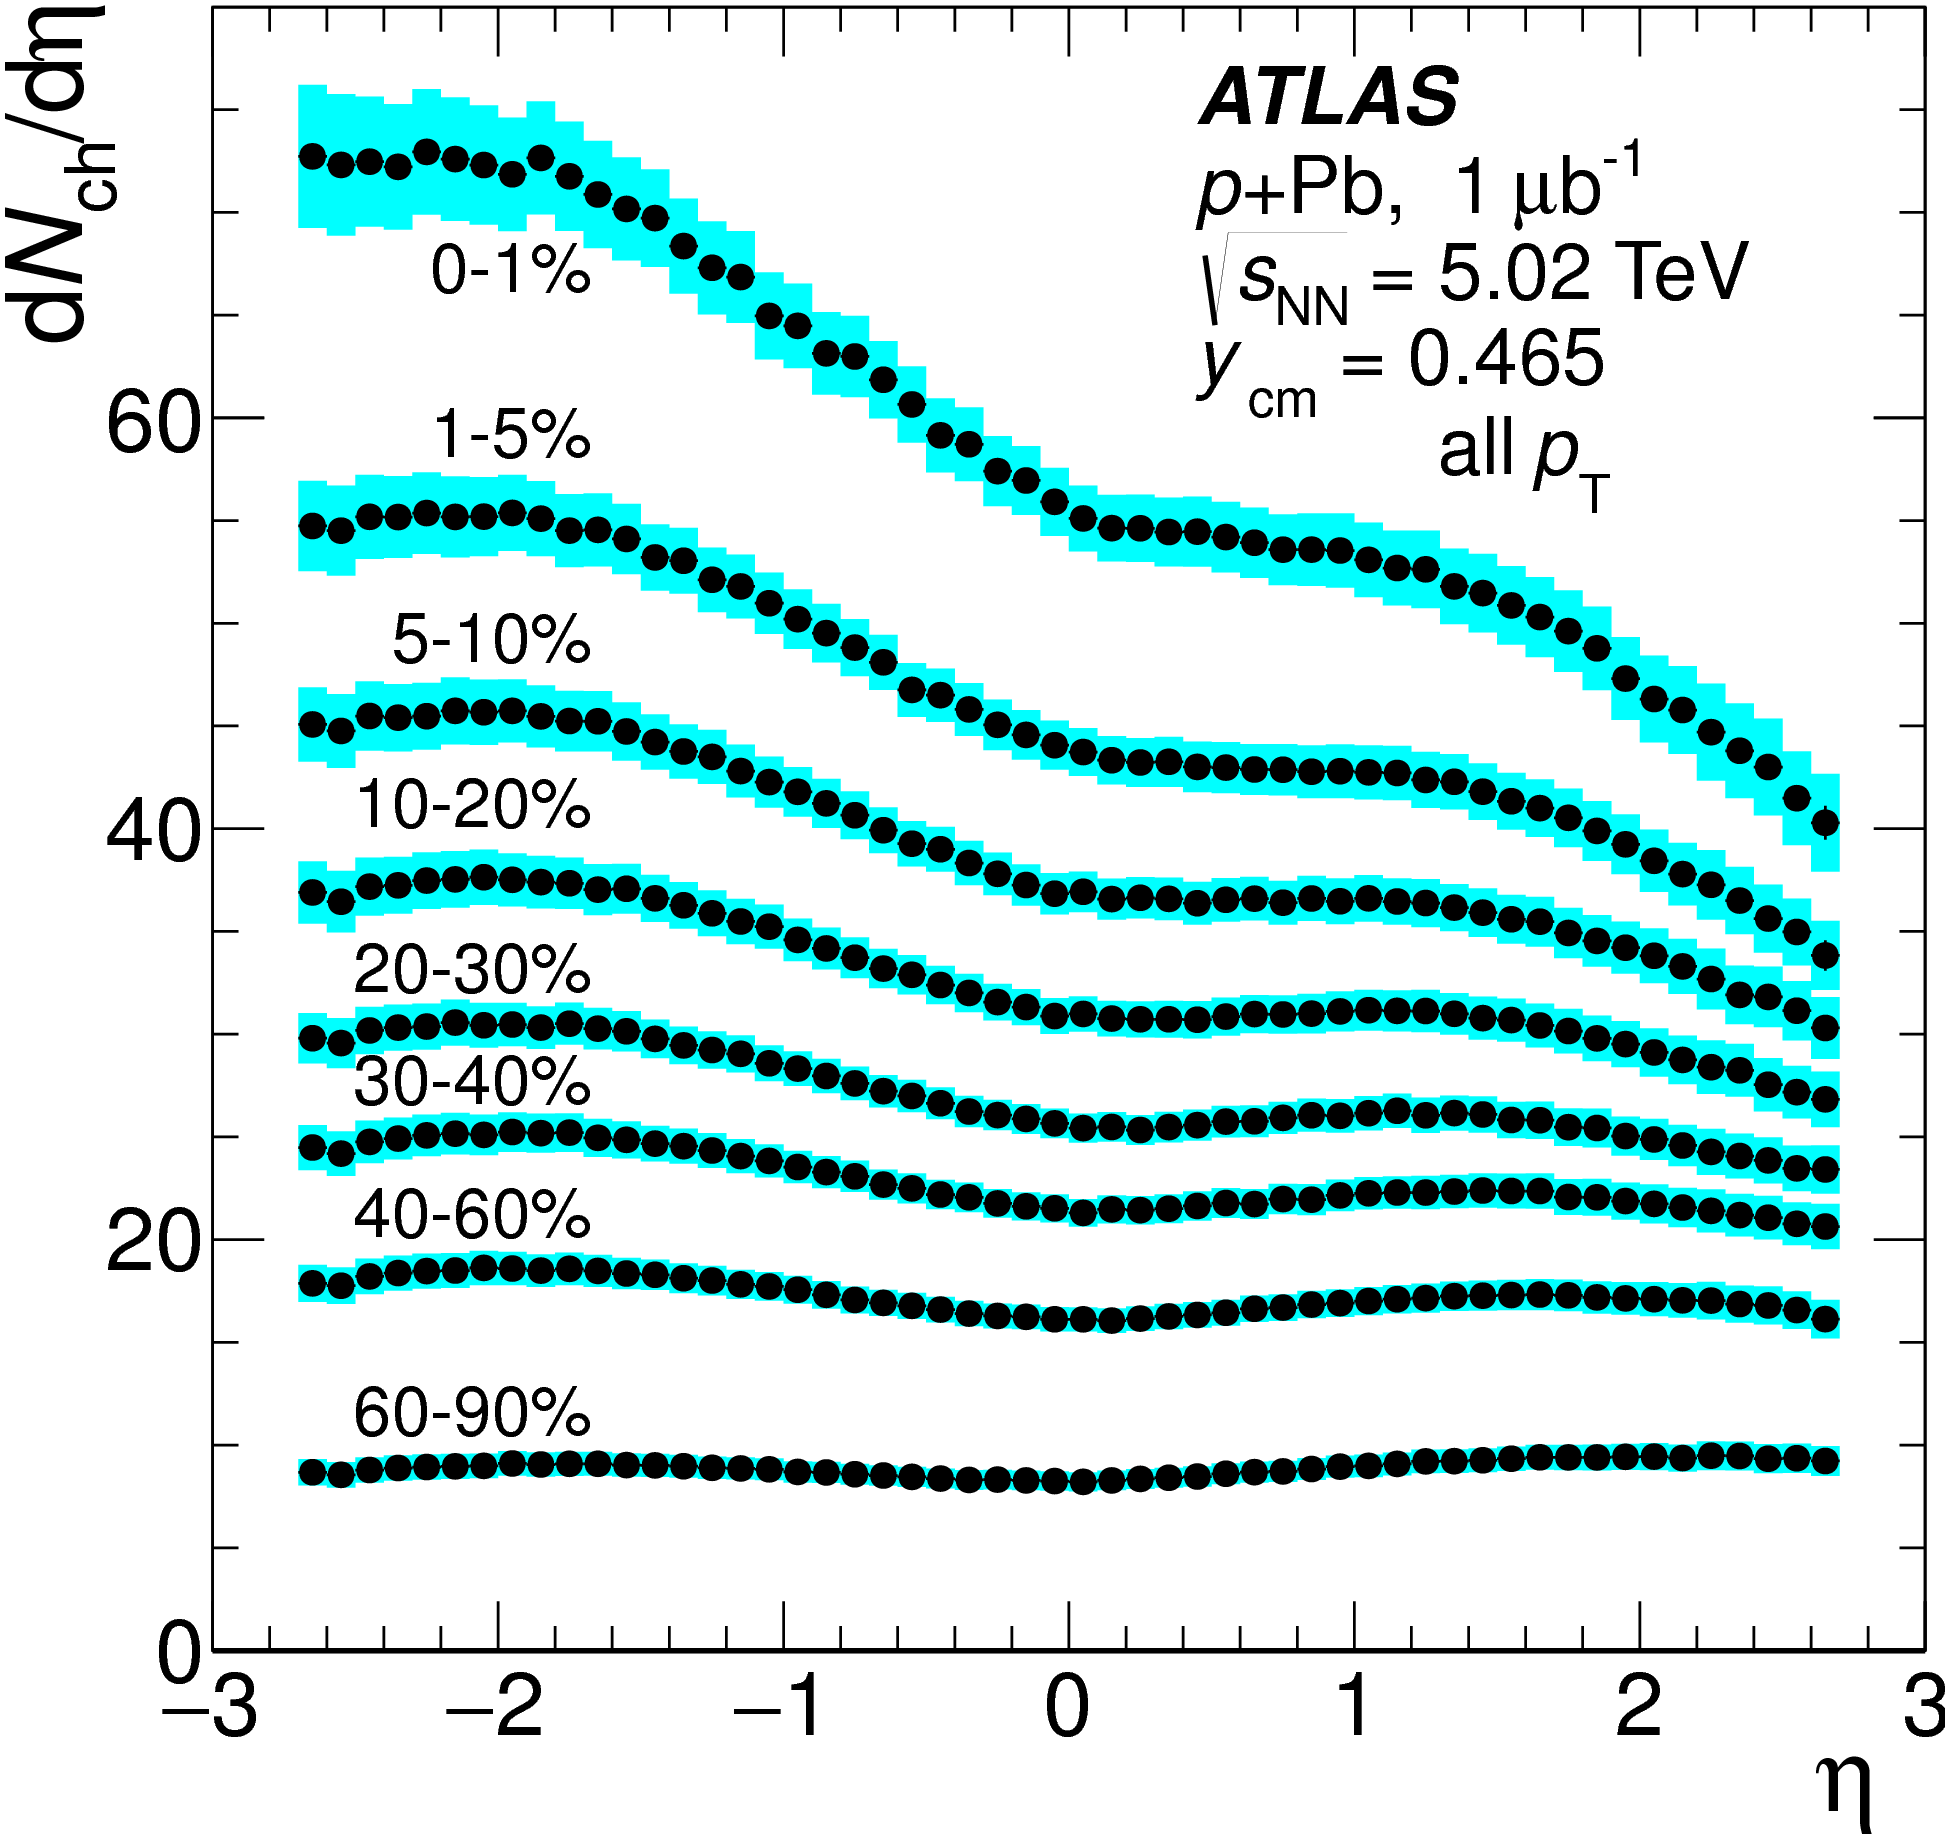
\includegraphics[width=0.33\textwidth]{pPb-ATLAS.png}\\
\end{overprint}
\hspace{9cm}\tiny EPJ C (2016) 76:199
\end{frame}


\section{Parametric longitudinal information}
\begin{frame}{A phenomenological model for 3D entropy production}
Start from \underline{midrapidity}: parametric model \TRENTo {\tiny PRC 92, 011901(2015)}.
\begin{itemize}
\item Nuclear thickness function, ${\color{blue} T_{A, B}(x_\perp)} = \int dz \rho_{A, B}^{}(z, x_\perp)$.
\end{itemize}

\begin{columns}
\begin{column}{0.65\textwidth}
\begin{itemize}
\item \TRENTo: mappings from ${\color{blue} T_A, T_B}$ to \underline{midrapidity} entropy production,
\begin{eqnarray}
\nonumber
s_0(x_\perp, \eta=0) \propto \left(\frac{{\color{blue} T_A}^{\color{red} p} + {\color{blue} T_B}^{\color{red} p}}{2}\right)^{1/{\color{red} p}}.
\end{eqnarray}
${\color{red} p}$: a tunable parameter. Let model mimic and interpolate between different initial condition models.
\end{itemize}
\end{column}
\begin{column}{0.35\textwidth}
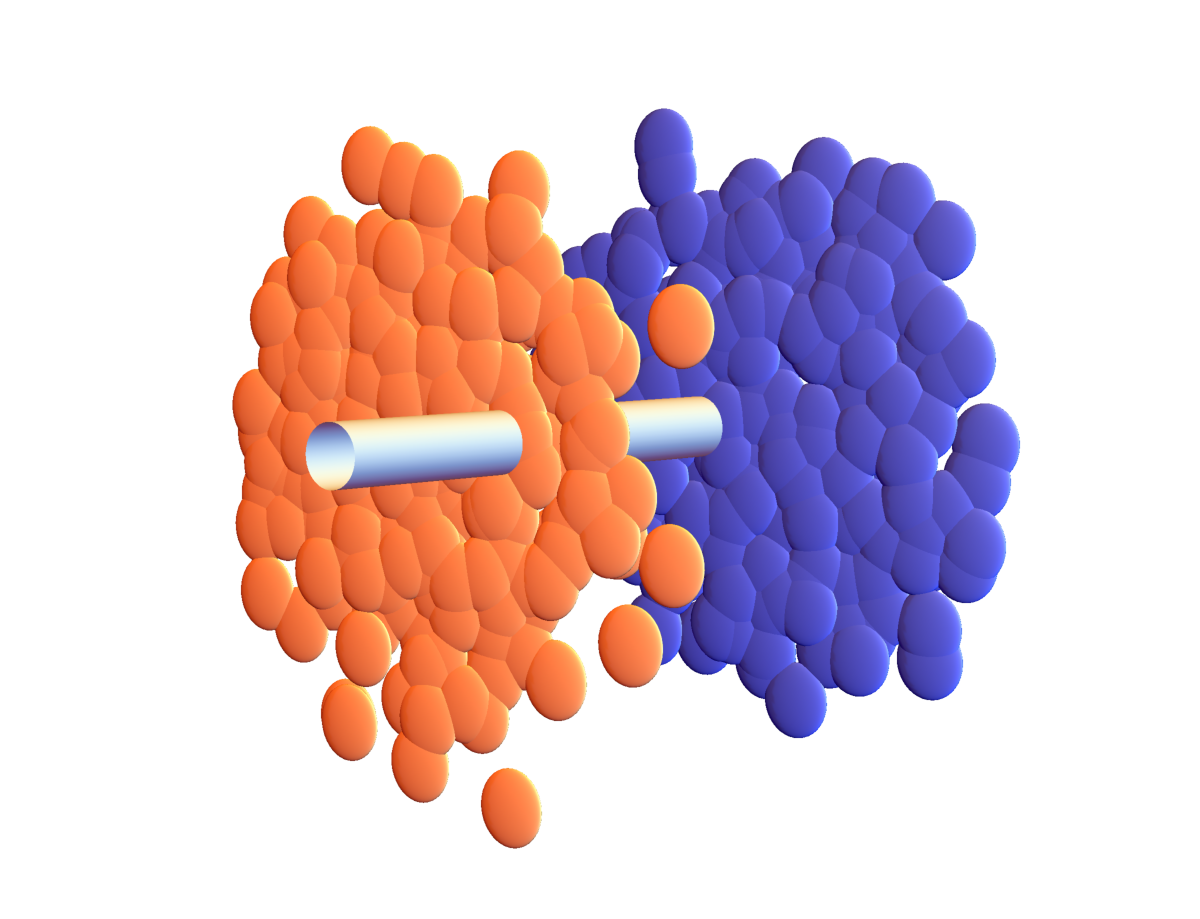
\includegraphics[width=\textwidth]{overlap_3.pdf}
\begin{center}
\tiny by J S Moreland
\end{center}
\end{column}
\end{columns}
\end{frame}

\begin{frame}{Extending \TRENTo to finite rapidity}
\begin{columns}
\begin{column}{0.7\textwidth}
\begin{eqnarray}
\nonumber 
\frac{dS}{dx_\perp^2d y} \propto
s_0(\vec{x}_\perp, y=0)  &\times&	{\color{orange}f(y, x_\perp)}.\\
\nonumber 
\textrm{ \TRENTo} &\times& \textrm{{\color{orange} rapidity profile}}
\end{eqnarray} 
\end{column}
\begin{column}{0.3\textwidth}
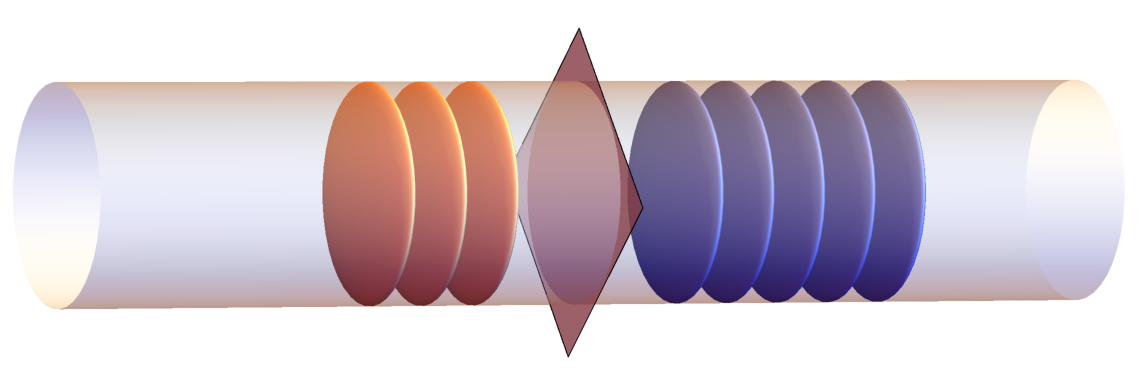
\includegraphics[width=\textwidth]{traincar-crop.pdf}
\end{column}
\end{columns}

\begin{itemize}
\item {\color{orange} $f(y, x_\perp)$} has three degrees of freedom (first 3 $y$-moments.):\\
\begin{center}
mean $\mu(x_\perp)$, std $\sigma(x_\perp)$, skewness $\gamma(x_\perp)$
\end{center}
\vspace*{-0.2cm}
\begin{eqnarray}\nonumber 
f(y, x_\perp) \propto \mathcal{F}^{-1}\exp\left\{i\mu k -\frac{1}{2}(\sigma k)^2 - \frac{i}{6}\gamma(\sigma k)^3 + ...\right\}
\end{eqnarray}
\item $\mu$, $\sigma$, $\gamma$ parametrized in nuclear thickness functions $T_A(x_\perp), T_B(x_\perp)$.
\end{itemize}
\begin{center}
\begin{tabularx}{0.8\textwidth}{p{2.3cm}p{1.2cm}p{6cm}}
\hline
mean ($\mu$) & std ($\sigma$) &$\left.\right.${\color{red!70}absolute} or {\color{blue!70}relative}-skew ($\gamma$) \\
\hline
\noalign{\smallskip}
$\frac{\mu_0}{2} \log\frac{T_A}{T_B}$ & $\sigma_0$ & $\left.\right.${\color{red!70}$\gamma_0(T_A-T_B)$} 
or 
{\color{blue!70}$\gamma_0\frac{T_A-T_B}{T_A+T_B}$} \\
\noalign{\smallskip}
\hline
\end{tabularx}
\end{center}
\end{frame}

\section{Model to data comparison}
\begin{frame}{Model-to-data comparison}
Model: T\raisebox{-0.2em}{R}ENTo-3D, 3+1D Hydro {\tiny (CPC 185 (2014), 3016)}, Ultra-relativistic Quantum Molecular Dynamics (UrQMD) {\tiny (Prog.Part.Nucl.Phys.41:255-369,1998)}


\begin{center}
Summary of parameters
\begin{tabular}{c|c}
\hline 
Transverse & normalization, nucleon size, fluctuation, $p$ \\ 
\hline 
Longitudinal & $\mu_0,\sigma_0, \gamma_0$, Jacobian \\ 
\hline 
\end{tabular} 
\end{center}

\begin{center}
Experimental data
\begin{tabularx}{0.8\textwidth}{p{4.5cm}|p{4cm}}
\hline
 Charged particle $\eta$-density & ALICE Pb+Pb 2.76 TeV ATLAS $p$+Pb 5.02 TeV \\ 
\hline
Two-particle $\eta$-correlation & ATLAS Pb+Pb 2.76 TeV \\
\hline
\end{tabularx}
\end{center}

Assuming viscous effects on the total multiplicity observables are mild, use ideal hydro as a first step.
\end{frame}

\begin{frame}{Bayesian model-to-data comparison}
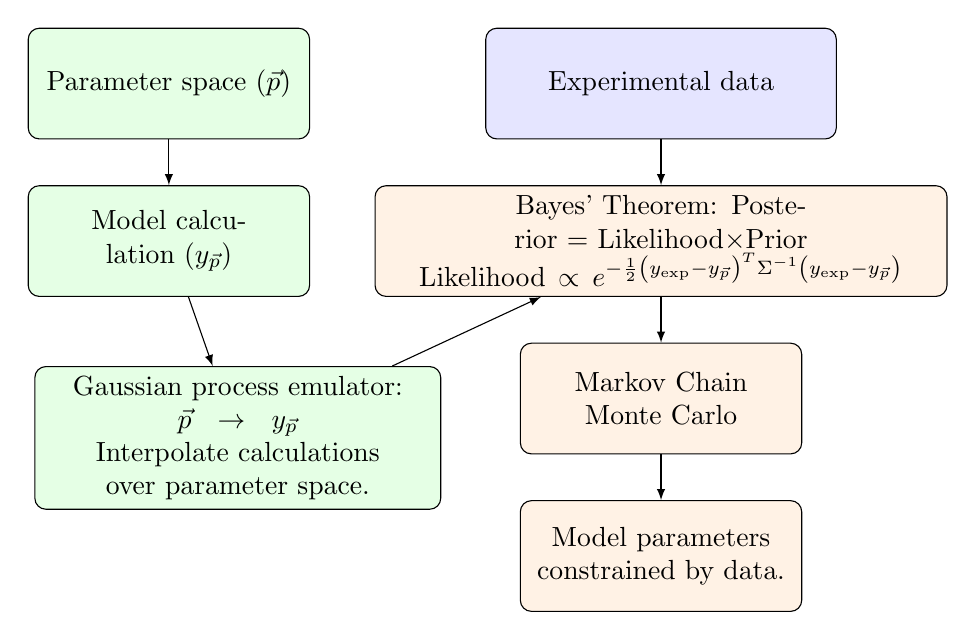
\begin{tikzpicture}[align=center,node distance=4cm]
    % Place nodes
    \node [block, fill=green!10] (param) {Parameter space ($\vec{p}$)};
    \node [block, fill=green!10, below of=param, yshift=2cm] (model) {Model calculation ($y_{\vec{p}}$)};
    \node [block, text width=12em, fill=blue!10, right of=param, xshift=2.25cm] (exp) {Experimental data};
    \node [block, text width=14em, fill=green!10, below of=model, xshift=0.875cm, yshift=1.5cm] (GP) {Gaussian process emulator: \\$\vec{p}\rightarrow y_{\vec{p}}$\\ Interpolate calculations over parameter space.};
    \node [block, text width=20em, fill=orange!10, right of=model, xshift=2.25cm] (Bayes) {
    Bayes' Theorem: Posterior = Likelihood$\times$Prior\\ 
    $\textrm{Likelihood} \propto e^{-\frac{1}{2} \left(y_{\textrm{exp}} - y_{\vec{p}} \right)^T \Sigma^{-1} \left(y_{\textrm{exp}} - y_{\vec{p}} \right)}$
    };
	\node [block, fill=orange!10, below of=Bayes, xshift=0.0cm, yshift=2cm] (MCMC) {Markov Chain Monte Carlo};
	\node [block, fill=orange!10, below of=MCMC, yshift=2cm] (posterior) {Model parameters constrained by data.};
    % Draw edges
    \path [line] (param)-- (model);
    \path [line] (model) -- (GP);
    \path [line] (GP) -- (Bayes);
    \path [line] (exp) -- (Bayes);
   	\path [line] (Bayes) -- (MCMC);
   	\path [line] (MCMC) -- (posterior);

\end{tikzpicture}
\end{frame}

\section{Constraint initial condition and predictions}
\begin{frame}{After fitting to data: posterior observables}
\begin{itemize}
\item Nicely fit the centrality $\&$ pseudorapidity dependence of $dN_{ch}/d\eta$.
\item  Initial condition + hydro approach for two particle $\eta$-correlation breaks down at large centrality.
\end{itemize}
\begin{center}
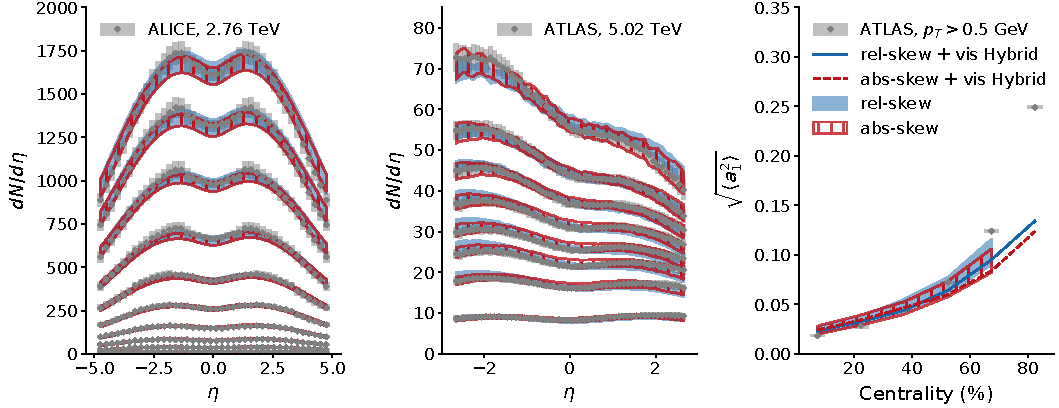
\includegraphics[width=\textwidth]{post_obs.pdf}\\
\tiny  	PLB 726 (2013) 610-622, PLB 754 (2016) 373-385, EPJ C (2016) 76:199, Nucl. Part. Phys. Proc. 276–278, 121 (2016).
\end{center}
\end{frame}

\begin{frame}{3D entropy production reverse engineered from data}

\begin{columns}
\begin{column}{0.55\textwidth}
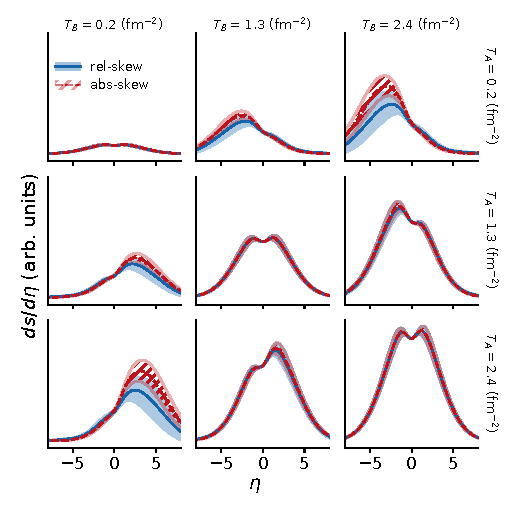
\includegraphics[width=\textwidth]{post_dsdy.pdf}
\end{column}
\begin{column}{0.45\textwidth}
\begin{itemize}
\item $ds/d\eta$ varies with $T_A$, $T_B$.
\item Imbalance \& fluctuations of $T_A$, $T_B$ lead to asymmetric local entropy production.
\item What's still missing: early time dynamical fluctuations.
\end{itemize}
\end{column}
\end{columns}

\end{frame}

\begin{frame}{Apply to $\eta$-dependent azimuthal correlations.}
Select high probability parameters. Use viscous hydro ($\eta/s \sim 0.25$) + UrQMD to calculate $v_n\{2\}$, $v_2\{4\}$, event-plane decorrelations.
\begin{center}
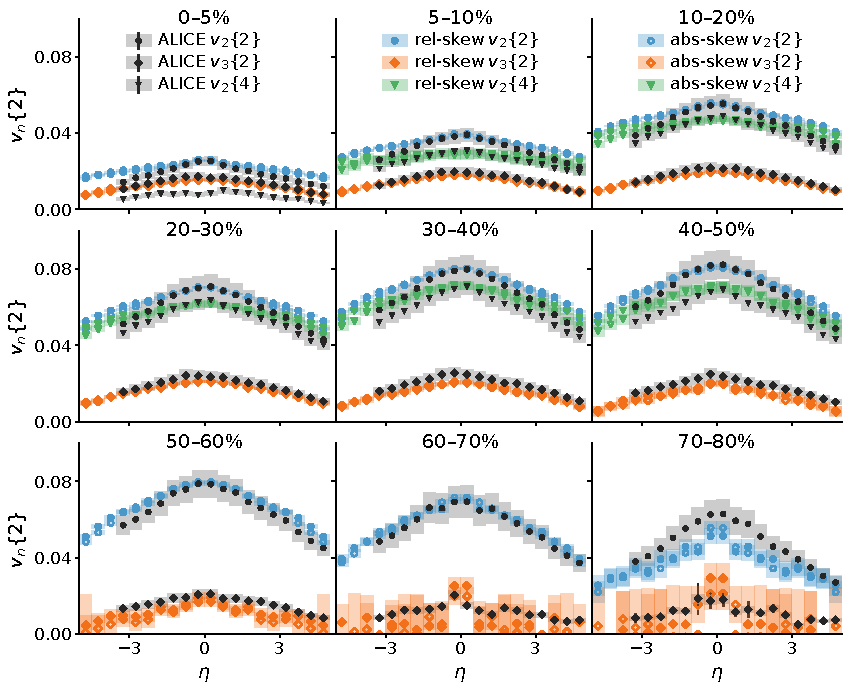
\includegraphics[width=0.59\textwidth]{vn_eta.pdf}\quad
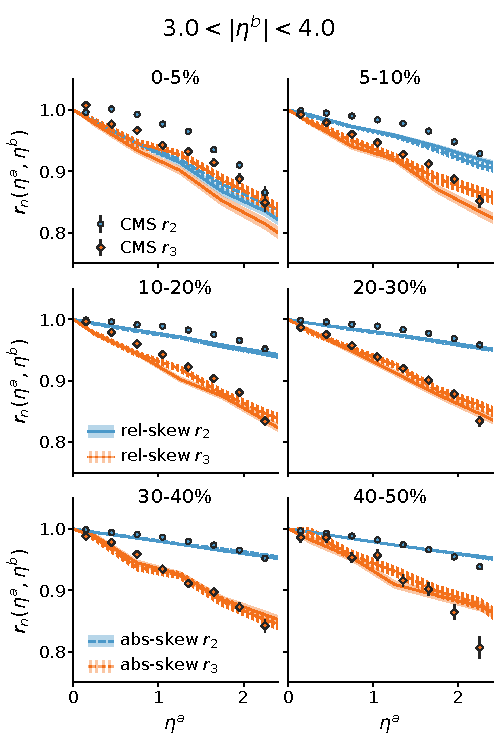
\includegraphics[width=0.325\textwidth]{evt_pln_decorr_near.pdf}\\
\tiny PLB 762 (2016) 376-388, PRC 92 (2015) 034911
\end{center}
\end{frame}

\begin{frame}{Summary}
\begin{itemize}
\item \TRENTo is extended to include rapidity dependence.
\vspace*{0.5cm}
\item Experimental data over-constrains the model parameters.
\vspace*{0.5cm}
\item \colorbox{red!20}{Initial 3D entropy production reverse engineered
 from experiments.}
\vspace*{0.5cm}
\item \colorbox{blue!20}{Provide guidance for first principal calculation.}
\vspace*{0.5cm}
\item \colorbox{blue!20}{Could benefit small system simulations.}
\end{itemize}
\end{frame}

\begin{frame}[noframenumbering]{Back up: full nine-parameter posterior}
\begin{center}
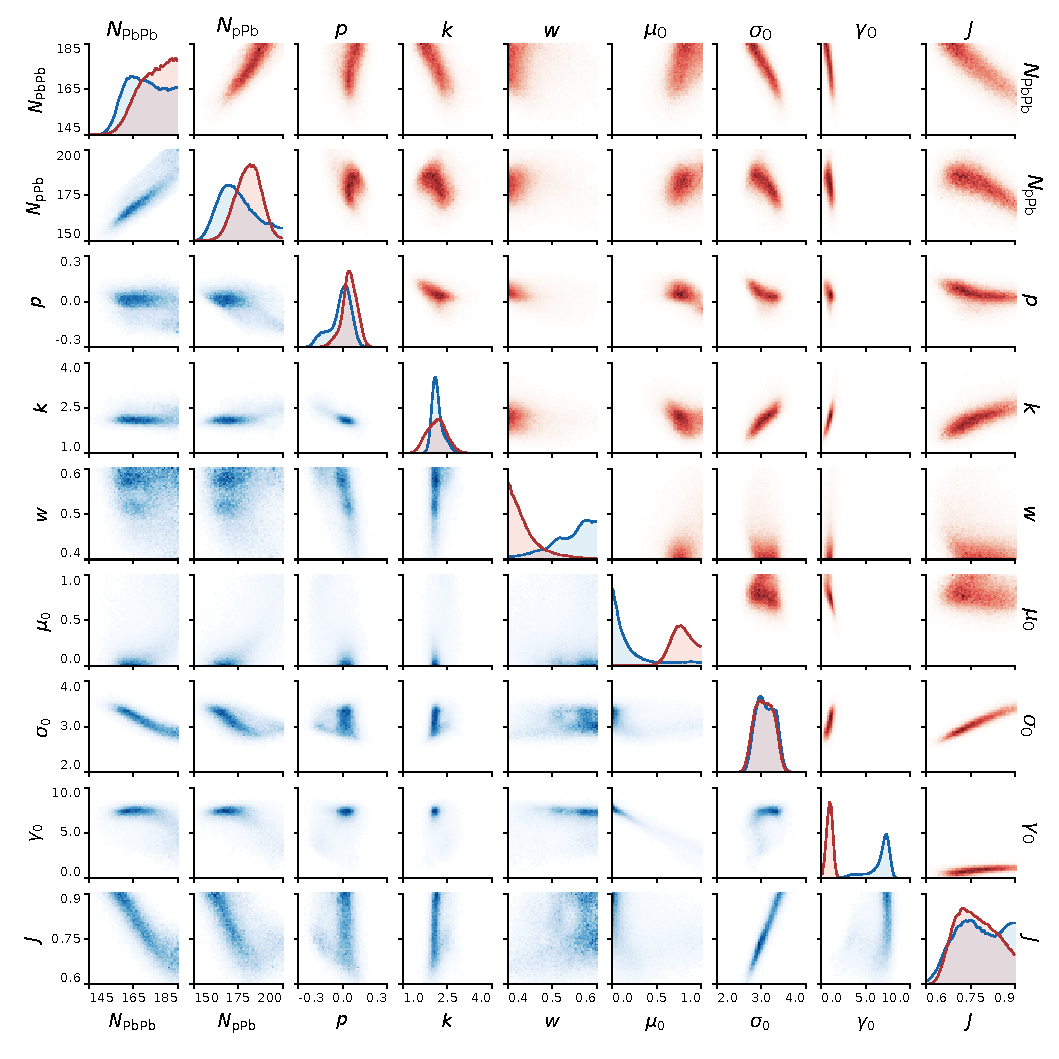
\includegraphics[width=0.7\textwidth]{posterior.pdf}
\end{center}
\end{frame}

\begin{frame}[noframenumbering]{Back up: Flow at midrapidity}
\begin{center}
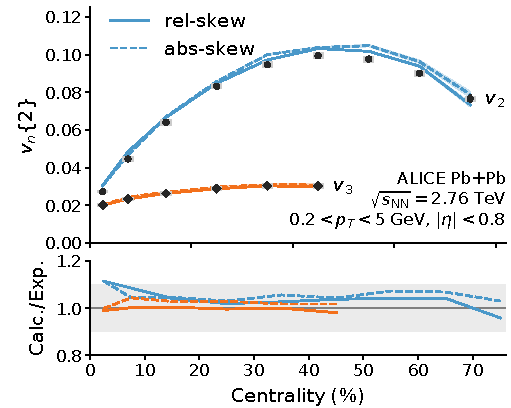
\includegraphics[width=0.8\textwidth]{vn_cen.pdf}
\end{center}
\end{frame}

\begin{frame}[noframenumbering]{Back up: event-plane decorrelation}
\begin{center}
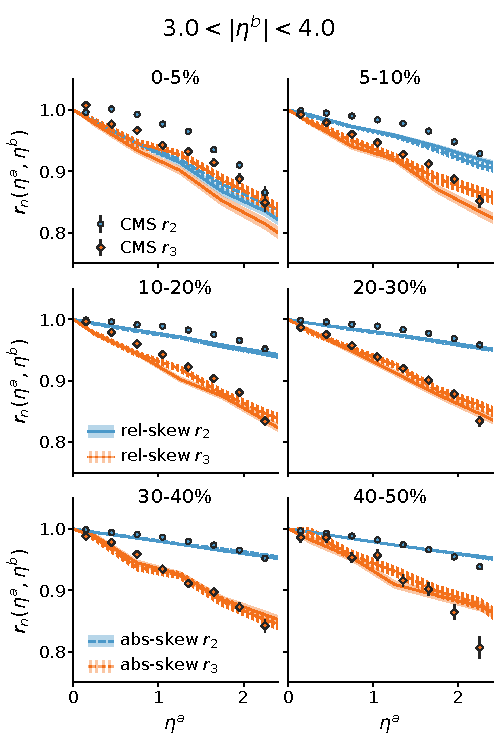
\includegraphics[width=0.45\textwidth]{evt_pln_decorr_near.pdf}
\quad\quad
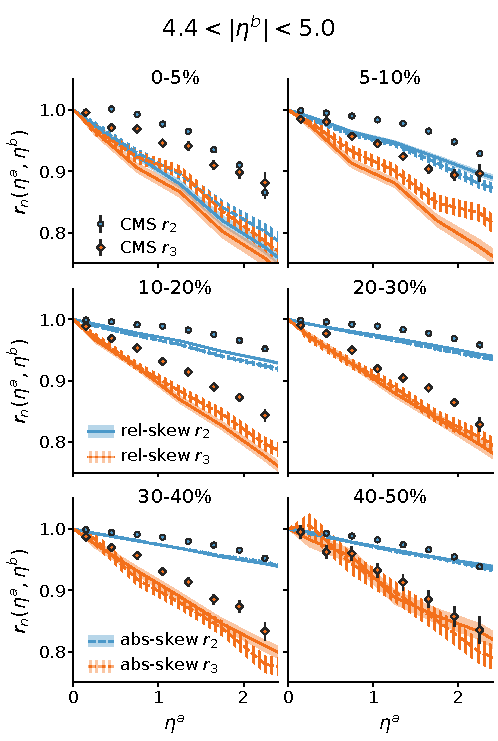
\includegraphics[width=0.45\textwidth]{evt_pln_decorr_far.pdf}
\end{center}
\end{frame}

\begin{frame}[noframenumbering]{Back up: calculation of symmetric cumulants}
\begin{center}
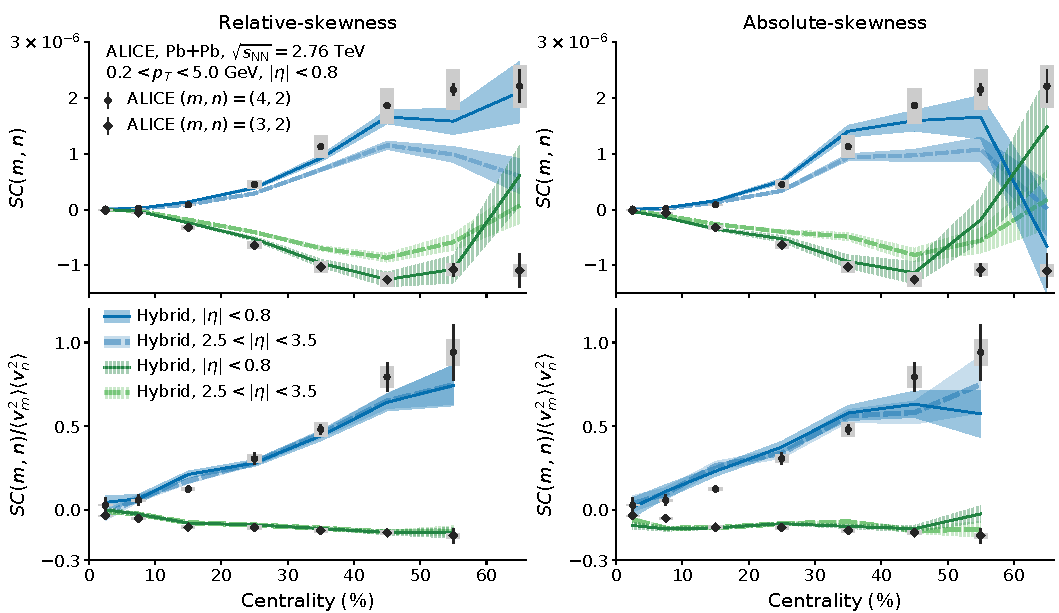
\includegraphics[width=\textwidth]{smn.pdf}
\end{center}
\end{frame}

\begin{frame}[noframenumbering]{Back up: Inverse the cumulant generating function}
To ensure the function inversed from cumulant generating function has good properties, 
\begin{eqnarray}
&-3.3\sigma < y < 3.3\sigma, \\
&\gamma \rightarrow \gamma\exp\left(-\frac{1}{2}\sigma^2k^2\right).
\end{eqnarray}
\begin{center}
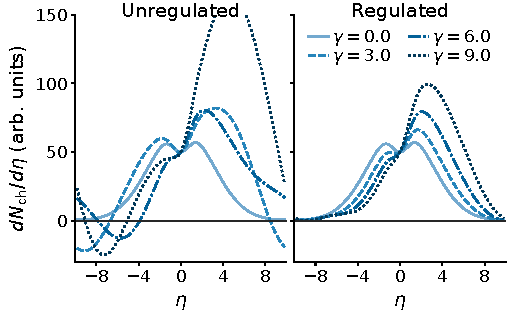
\includegraphics[width=0.7\textwidth]{regulate.pdf}
\end{center}
\end{frame}

\begin{frame}[noframenumbering]{Back up: Two particle $\eta$-correlation}
Expand event-wise $dN/d\eta$ in Legendre Polynomials (within $|\eta|<Y$). 
\begin{eqnarray}
\nonumber
\frac{dN}{d\eta} = \left\langle \frac{dN}{d\eta} \right\rangle \left(a_0 + a_1 P_1\left(\frac{\eta}{Y}\right) + a_2 P_2\left(\frac{\eta}{Y}\right) + ...\right)
\end{eqnarray}
The correlations between the expansion coefficients are related to the two particle $\eta$-correlation function,
\begin{eqnarray}
\nonumber
C(\eta_1,\eta_2) &=& \frac{\left\langle dN(\eta_1)dN(\eta_2)\right\rangle}{\left\langle dN(\eta_1)\right\rangle\left\langle dN(\eta_2)\right\rangle}-1\\
\nonumber
\left\langle a_n a_m\right\rangle &=& \frac{(2n+1)(2m+1)}{4} \int \frac{d\eta_1}{Y}\frac{d\eta_2}{Y} C(\eta_1,\eta_2)T_{mn}(\eta_1,\eta_2)\\
T_{mn}(1,2) &=& \frac{P_m(1)P_n(2)+P_m(2)P_n(1)}{2}
\end{eqnarray}
\end{frame}


\end{document}
